\chapter{Практические задания}
\section{Составить диаграмму вычисления следующих выражений:}

\begin{enumerate}
	\item (equal 3 (abs -3))
	\begin{figure}[H]
		\centering{
			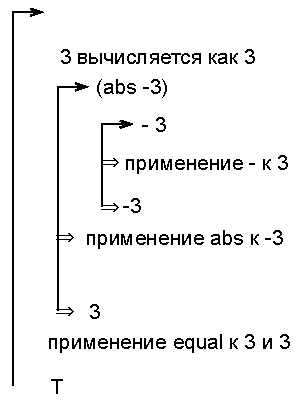
\includegraphics[scale=1]{images/task_1_1.pdf}}
	\end{figure}
	
	\item (equal (+ 1 2) 3)
	\begin{figure}[H]
		\centering{
			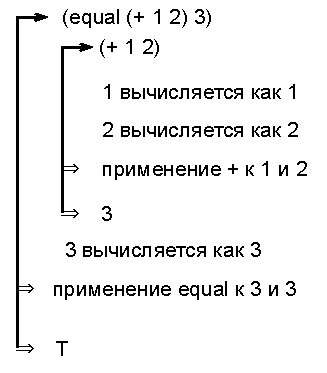
\includegraphics[scale=1]{images/task_1_2.pdf}}
	\end{figure}

	\newpage
	\item (equal (* 4 7) 21)
	\begin{figure}[H]
		\centering{
			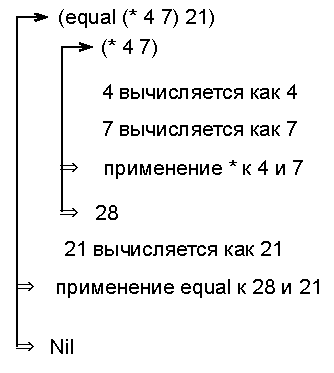
\includegraphics[scale=1]{images/task_1_3.pdf}}
	\end{figure}

	\item (equal (* 2 3) (+ 7 2))
	\begin{figure}[H]
		\centering{
			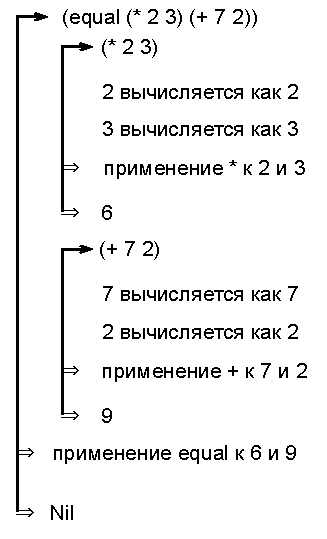
\includegraphics[scale=1]{images/task_1_4.pdf}}
	\end{figure}
	
	\newpage
	\item (equal (- 7 3) (* 3 2))
	\begin{figure}[H]
		\centering{
			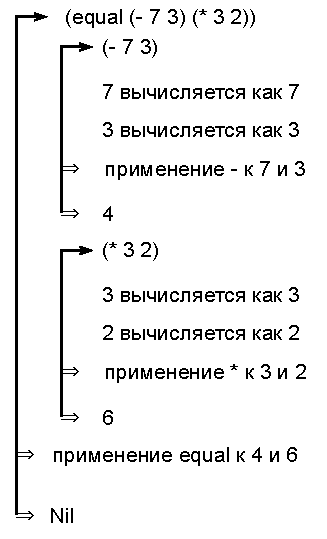
\includegraphics[scale=1]{images/task_1_5.pdf}}
	\end{figure}

	\item (equal (abs (- 2 4) 3)) 
	\begin{figure}[H]
		\centering{
			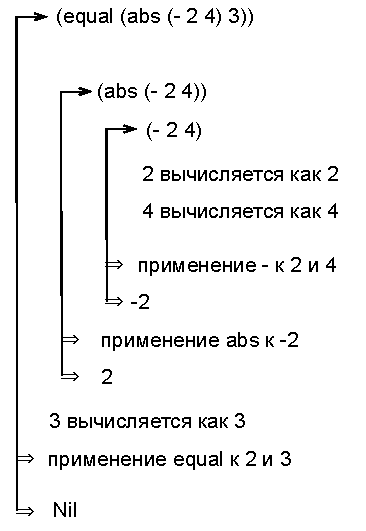
\includegraphics[scale=1]{images/task_1_6.pdf}}
	\end{figure}
\end{enumerate}

\section{Написать функцию, вычисляющую гипотенузу прямоугольного треугольника по заданным катетам и составить диаграмму её вычисления.}

\begin{lstlisting}[label=lst:task_2, caption=Задание 2.]
	(defun hypotenuse (cath1 cath2) 
		(sqrt (+ (* cath1 cath1) (* cath2 cath2))))
\end{lstlisting}

\begin{figure}[H]
	\centering{
		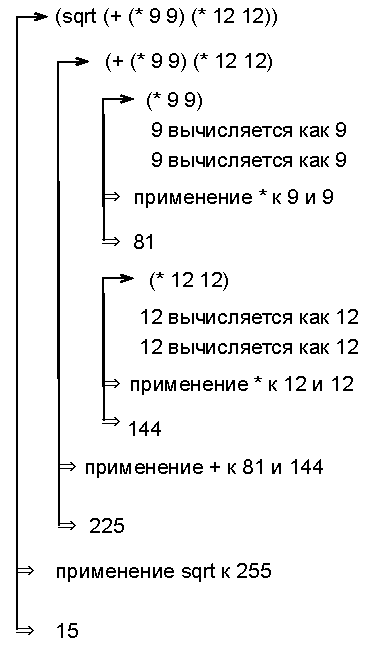
\includegraphics[scale=1]{images/task_2.pdf}}
\end{figure}

\newpage
\section{Написать функцию, вычисляющую объем параллелепипеда по трем его сторонам, и составить диаграмму ее вычисления.}

\begin{lstlisting}[label=lst:task_3, caption=Задание 3.]
	(defun volume (side1 side2 side3) (* side1 side2 side3))
\end{lstlisting}

\begin{figure}[H]
	\centering{
		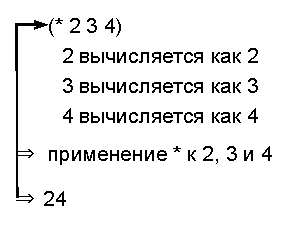
\includegraphics[scale=1]{images/task_3.pdf}}
\end{figure}

\section{Каковы результаты вычисления следующих выражений? Объяснить возможную ошибку и варианты ее устранения}
\begin{enumerate}
	\item (list 'a c)  ;ошибка $\Rightarrow$ (list 'a c)
	\item (cons 'a (b c)) ;ошибка $\Rightarrow$ (cons 'a '(b c))
	\item (cons 'a '(b c)) $\Rightarrow$ (a b c)
	\item (caddy (1 2 3 4 5)) ;ошибка $\Rightarrow$ (caddr (1 2 3 4 5)) $\Rightarrow$ ошибка $\Rightarrow$ 
	
	\hspace{4.5cm};(caddr '(1 2 3 4 5))
	\item (cons 'a 'b 'c)  ;ошибка $\Rightarrow$ (cons 'a '('b 'c))
	\item (list 'a (b c))  ;ошибка $\Rightarrow$ (list 'a '(b c))
	\item (list a '(b c))  ;ошибка $\Rightarrow$ (list 'a (b c))
	\item (list (+ 1 '(length '(1 2 3)))) ;ошибка $\Rightarrow$ (list (+ 1 (length '(1 2 3))))
\end{enumerate}

\section{Написать функцию longer\_then от двух списков-аргументов, которая возвращает Т, если первый аргумент имеет большую длину.}

\begin{lstlisting}[label=lst:task_5, caption=Задание 5.]
	(defun longer_then (arg1 arg2) (>= (length arg1) (length arg2)))
\end{lstlisting}

\section{Каковы результаты вычисления следующих выражений?}

\begin{enumerate}
	\item (cons 3 (list 5 6)) $\Rightarrow$ (3 5 6)
	\item (cons 3 '(list 5 6)) $\Rightarrow$ (3 list 5 6)
	\item (list 3 'from 9 'lives (- 9 3)) $\Rightarrow$ (3 from 9 lives 6)
	\item (+ (length for 2 too)) (car '(21 22 23))) $\Rightarrow$ ошибка 
	\item (cdr '(cons is short for ans)) $\Rightarrow$ (is short for ans)
	\item (car (list one two)) $\Rightarrow$ ошибка
	\item (car (list 'one 'two)) $\Rightarrow$ one
\end{enumerate}

\newpage
\section{Дана функция (defun mystery (x) (list (second x) (first x))). Какие результаты вычисления следующих выражений?}
\begin{enumerate}
	\item (mystery (one two)) $\Rightarrow$ ошибка
	\item (mystery (last one two)) $\Rightarrow$ ошибка
	\item (mystery free) $\Rightarrow$ ошибка
	\item (mystery one 'two)) $\Rightarrow$ ошибка
\end{enumerate}

\section{Написать функцию, которая переводит температуру в системе Фаренгейта температуру по Цельсию (defun f-to-c (temp)…).}

Формулы:

\begin{enumerate}
	\item $c = 5/9*(f-320)$;
	\begin{lstlisting}[caption=Перевод из Фаренгейт в Цельсий.]
	(defun f_to_c (temp) (* (/ 5 9) (- temp 32.0)))
	\end{lstlisting}
	
	\item $f = 9/5*c+32.0$;
	\begin{lstlisting}[caption=Перевод из Цельсия в Фаренгейт.]
	(defun c_to_f (temp) (+ (* (/ 9 5) temp) 32.0))
	\end{lstlisting}
\end{enumerate}

Как бы назывался роман Р.Брэдбери <<+451 по Фаренгейту>> в системе по Цельсию? 
<<+232.778 по Цельсию>>

\newpage
\section{Что получится при вычислении каждого из выражений?}
\begin{enumerate}
	\item (list 'cons t NIL) $\Rightarrow$ (cons t Nil)
	\item (eval (list 'cons t NIL))
	
	(eval (cons t Nil)) 
	
	(eval (t)) $\Rightarrow$ ошибка
	
	\item (eval (eval (list 'cons t NIL)))
	
	(eval (eval (cons t Nil)))
	
	(eval (eval (t))) $\Rightarrow$ ошибка
	
	\item (apply \#cons ''(t NIL)) $\Rightarrow$ ошибка
	
	(apply \#'cons '(t NIL)) $\Rightarrow$ (t)
	
	\item (list 'eval NIL) $\Rightarrow$ (eval NIL)
	\item (eval NIL) $\Rightarrow$ Nil
	\item (eval (list 'eval NIL)) $\Rightarrow$ Nil
\end{enumerate}

\newpage
\section*{Дополнительные задания}
\section{Написать функцию, вычисляющую катет по заданной гипотенузе и другому катету прямоугольного треугольника, составить диаграмму ее вычисления.}

\begin{lstlisting}[caption=Дополнительное задание 1.]
	(defun hypo_cath (hypo cath) 
		(sqrt (- (* hypo hypo) (* cath cath))))
\end{lstlisting}

\begin{figure}[H]
	\centering{
		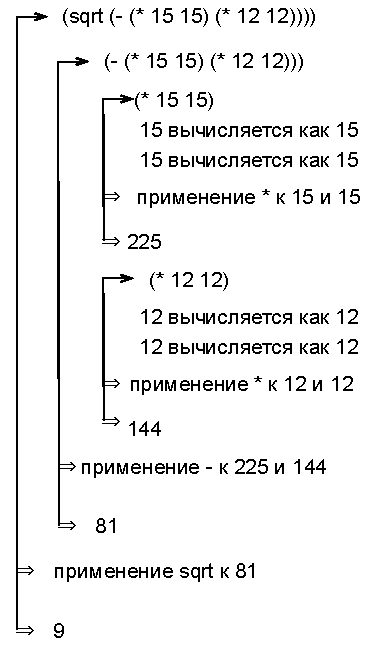
\includegraphics[scale=1]{images/dop_task_1.pdf}}
\end{figure}

\section{Написать функцию, вычисляющую площадь трапеции по ее основаниям и 	высоте, составить диаграмму ее вычисления.}

\begin{lstlisting}[caption=Дополнительное задание 2.]
	(defun trapezoid_square (base1 base2 height) 
		(* 0.5 (+ base1 base2) height))
\end{lstlisting}

\begin{figure}[H]
	\centering{
		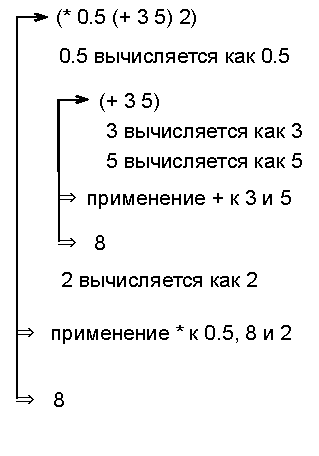
\includegraphics[scale=1]{images/dop_task_2.pdf}}
\end{figure}
